
% ----------------------------------------------------------------------
\introduction
\label{sec:intro}
% ----------------------------------------------------------------------

The numerical modelling of past glaciers and ice sheets allows indirect confrontation between glaciological theories and geomorphological reconstructions, challenging the validity of both. Yet a major obstacle in this exercise resides in the large uncertainties that affect climate forcing of numerical glacier models \citep{hebeler-etal-2008}. This includes the uncertainty on Earth's present climate, and the larger uncertainty on its changes in the past.

Numerical models of the former North American ice sheets have used various climate forcing methods, ranging from simplistic parametrizations to coupling to General Circulation Models (GCM). The latter is arguably the most physically sound way to force an ice sheet model in the past and has proven effective \citep{yoshimori-etal-2001,calov-etal-2002,abeouchi-etal-2007,charbit-etal-2013}. However the computational demand of GCMs is so that only models of reduced complexity and coarser resolution can run on time-scales of ice sheet growth and decay.

Another method consist in using atmospheric fields produced in uncoupled palæo-climate simulations \citep{huybrechts-tsiobbel-1996}. To produce a time-dependant forcing, the GCM output is interpolated in time between different simulations \citep{charbit-etal-2002} or weighted based on ice-core records \citep{marshall-clarke-1999,tarasov-peltier-2004,zweck-huybrechts-2005,gregoire-etal-2012}. These palæo-climate simulations use ice sheet reconstructions such as the ICE-4G \citep{peltier-1994} as topographic boundary condition, which results in subsequently modelled ice cover consistent with these reconstructions.
\julien[noline]{Should this literature list be extended to studies not covering North America?}

%TODO tarasov-peltier-1997

Avoiding this circular dependence unfortunately goes with simplistic assumptions on Earth's past climate. \citet{robert-1991} use a parametrization of glacier surface mass balance based on elevation. \citet{fastook-prentice-1994} use a parametrization of climate forcing based on elevation and distance from a climatic pole initially prepared for Antarctica \citep{johnson-fastook-2002}. Finally, \citet{bintanja-etal-2005} apply time-dependant temperature offsets to a reference present-day climate obtained from climate reanalysis data. We use a similar method.

\begin{figure}[t]
	\vspace*{2mm}
	\begin{center}
		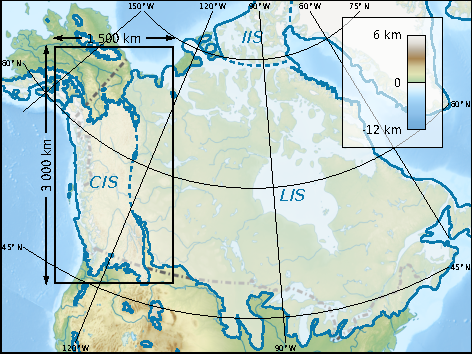
\includegraphics[width=8cm]{cordillera-climate-locmap}
	\end{center}
	\caption{Shaded relief map of northern North America. The frame delimits this study's modelling domain. The outlines of the former ice sheets depict ice cover at 14\,$^{14}$C\,ka\,BP (16.8\,cal\,ka\,BP) after \citet{dyke-2004}. The background map was made with ETOPO1 \citep{data:etopo1} and Natural Earth Data \citep{data:naturalearth}.}
	\label{fig:locmap}
\end{figure}

Our area of focus for the present study is the Cordilleran Ice Sheet in north-western North America (Figure 1). In a numerical modelling perspective, it is one of the least studied palæo-ice sheets of the Northern Hemisphere, where nevertheless significant geomorphological data is available \citep{jackson-clague-1991}. Although generally not the primary target of these simulations, the Cordilleran Ice Sheet has been previously modelled as part of the North American ice sheet complex \citep{marshall-clarke-1999,calov-etal-2002,tarasov-peltier-2004,bintanja-etal-2005,gregoire-etal-2012} and within a larger-scale Arctic or Global numerical domain \citep{huybrechts-tsiobbel-1996,charbit-etal-2002,johnson-fastook-2002,zweck-huybrechts-2005,abeouchi-etal-2007,charbit-etal-2013}.

While these studies reproduce well the magnitude of the North American glaciation at Last Glacial Maximum, they tend to predict excessive ice cover in parts of northern Yukon Territory and Alaska that have remained ice-free throughout the Pleistocene \citep{dukrodkin-1999,kaufman-manley-2004}.

Here we use a Parallel Ice Sheet Model \citep[PISM,][]{web:pism} to simulate the entire Cordilleran Ice Sheet at the Last Glacial Maximum (LGM). We force our model with multiple climate datasets and compare our results to the mapped LGM ice sheet margin from \citet{dyke-2004}. See \citet{quiquet-etal-2012} for a similar comparison on Greenland. To avoid any dependence on ice-sheet reconstructions and allow high spatial resolution in our climate forcing, we use present-day climate data and given temperature offsets in a manner similar to \citet{bintanja-etal-2005}. To our knowledge, this is the first modelling study which specifically focus on the Cordilleran Ice Sheet since the one by \citep{robert-1991}, who focused specifically on its southern margin.

